\section{Using policy languages to specify access control conditions}
\label{sec:sota_policies}
%everything copied from languages+vocabs_review, needs to be updated
Policy languages have been used in the last decades to specify information regarding the usage of data, e.g., to represent licenses associated with datasets or software usage.
As such, they seem perfectly aligned with the goal of representing the conditions to access data on the Web, whether being preferences set by data subjects or access requests from other entities.
In addition, if used together with privacy and data protection-specific terms, e.g., coming from the ontologies described in the previous Section, they can be used to model legally-aligned access control policies.

In the following Sections, the criteria used to analyse each specified policy language are described, as well as a description of each identified language.

\subsection{Criteria for analysis}
\label{sec:sota_policies_criteria}

% below copied
For each solution, there is an introductory summary of the language complemented by a description of its main contributions, followed by a description of the core elements of the language. When available, specific examples of use cases using the language are mentioned, as well as implementations derived from it, including details on any available reasoners that use the work. The dependencies of the solutions in previously existing works are also documented when described in the literature. In Table \ref{tab:resources-policy-languages}, there is a brief description of the policy languages specified in the subsequent Sections, \ref{sec:p3p} to \ref{sec:lpl}, including information about the creators of the resources, version, date of publication and date of the last known update. These solutions are analysed in chronological order in relation to the date of publication and then in relation to the date of the last update. In Figure \ref{fig:lang-dependency-graph}, a dependency graph, that captures the relations between languages and their dependencies and follow-up works, is presented.

Moreover, the following criteria were used to analyse existing research on semantic policy languages:
\begin{enumerate}
    \item[(C1)] Ability to model deontic concepts, e.g., permissions, prohibitions, obligations.
    \item[(C2)] Ability to model GDPR concepts, such as the privacy terms in Table \ref{tab:GDPR_privacy_terms}.
    \item[(C3)] Existence of taxonomies of terms to populate policy conditions.
    \item[(C4)] Existence of mechanisms to assist with compliance.
    \item[(C5)] Resource is maintained/continues to be actively developed.
    \item[(C6)] Existence of an open and accessible specification.
\end{enumerate}

The outcomes of this comparative analysis will be provided in Section \ref{sec:sota_policies_analysis} and systematised in Table \ref{tab:languagesComparison}.

\subsection{Semantic policy languages for access control}
\label{sec:sota_policies_description}

In this Section, we aim to identify privacy-related policy languages, describing the structure and information provided by each language as well as identify its compatibility with the GDPR to describe not only rights but also obligations. % copied
Moreover, Table \ref{tab:resources-policy-languages} provides an overview of these languages and collects information about the creators of the resources, their versions, the date of publication and the date of the last known update.
Said languages are then analysed in chronological order regarding the date of publication and a dependency graph is presented in Figure \ref{fig:lang-dependency-graph}.

\begin{table}
\centering
\caption{Brief description of the policy languages described in Section \ref{sec:sota_policies_description}.}
\label{tab:resources-policy-languages}
\resizebox{\textwidth}{!}{%
\begin{tabular}{c||c|c|c|c|c}
Abbreviation (Section) & Full Name & Creators & Version & \multicolumn{1}{c|}{\begin{tabular}[c]{@{}c@{}} Date of \\ publication \end{tabular}} & \multicolumn{1}{c}{\begin{tabular}[c]{@{}c@{}} Last \\ update \end{tabular}} \\
 \hline\hline
 P3P (\ref{sec:p3p}) & Platform for Privacy Preferences & Cranor et al. & 1.0 & 1998 & 2010 \\
 \hline
 ODRL (\ref{sec:odrl}) & Open Digital Rights Language & Iannella et al. & 2.2 & 2001 & 2019 \\
 \hline
 XPref (\ref{sec:xpref}) & XPath-based Preference Language & Agrawal et al. & - & 2003 & - \\
 \hline
 AIR (\ref{sec:air}) & Accountability In RDF & Khandelwal et al. & - & 2007 & 2009 \\
 \hline
 S4P (\ref{sec:s4p}) & SecPAL for Privacy & Becker et al. & - & 2009 & 2010 \\
 \hline
 POL (\ref{sec:pol}) & Privacy Option Language & Stefan Berthold & - & 2010 & 2013 \\
 \hline
 PPO (\ref{sec:ppo})& Privacy Preference Ontology & Sacco and Passant & - & 2011 & 2013 \\
 \hline
 LegalRuleML (\ref{sec:legalruleml}) & LegalRuleML Core Specification & Palmirani et al. & 1.0 & 2012 & 2021 \\
 \hline
 A-PPL (\ref{sec:appl}) & Accountable Policy Language & Azraoui et al. & - & 2013 & 2016 \\
 \hline
 P2U (\ref{sec:p2u}) & Purpose-To-Use & Iyilade and Vassileva & - & 2014 & - \\
 \hline
 SPL (\ref{sec:special}) & SPECIAL Usage Policy Language & Bonatti et al. & 1.0 & 2017 & 2019 \\
 \hline
 DPF (\ref{sec:dpf}) & Declarative Policy Framework & Martiny et al. & - & 2018 & 2020 \\
 \hline
 LPL (\ref{sec:lpl}) & Layered Privacy Language & Gerl et al. & - & 2018 & 2019 \\
\end{tabular}}
\end{table}

\begin{figure}
\caption{Privacy-related policy languages dependency chart.}
\label{fig:lang-dependency-graph}
\centering
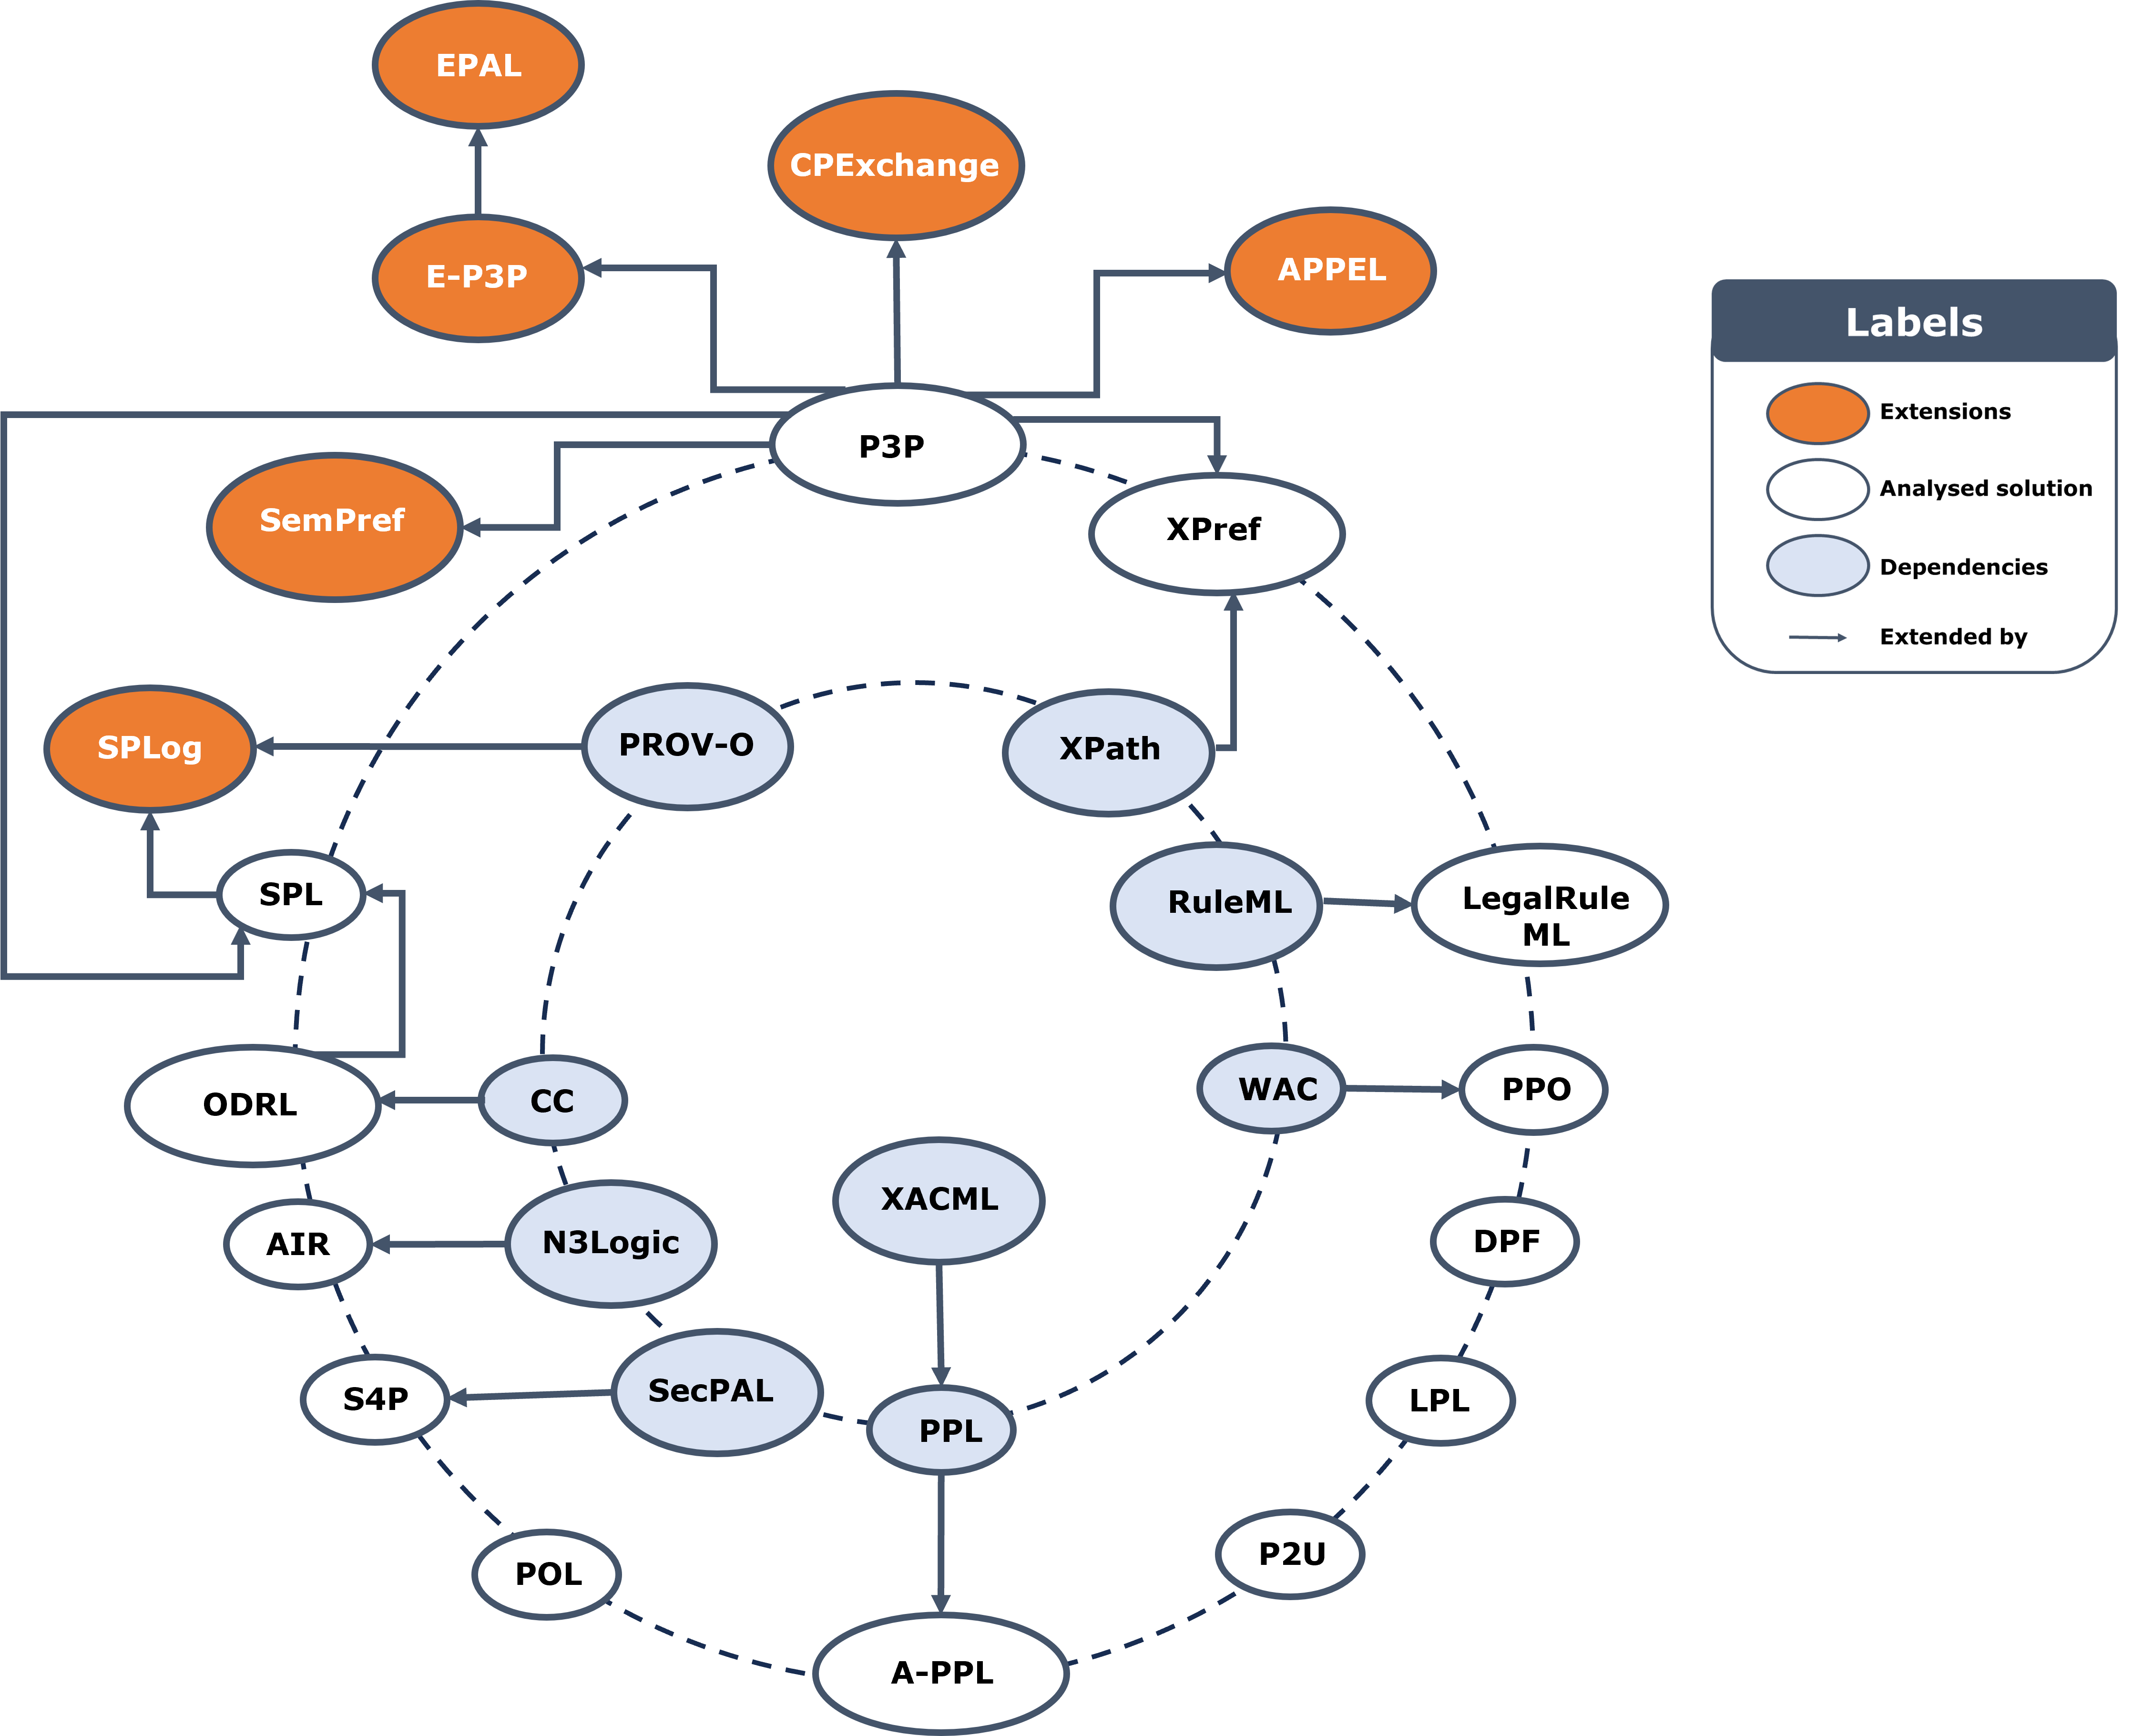
\includegraphics[width=\textwidth]{figures/chapter-2/languages.png}
\end{figure}

To complement the description of the languages presented in this Section, additional documentation and resources were published on a Web page\footnote{Available at \url{https://protect.oeg.fi.upm.es/sota/languages}. Its public repository can be consulted at \url{https://github.com/besteves4/SotAResources} for further improvement when new solutions appear.}, including diagrams and code examples.

% BPR4GDPR: 
% Using this ontology, BPR4GDPR defines a policy instantiating its purpose, context, action, pre-action and pos-action.
% The action reflects the activity permitted, prohibited or obliged by the policy, while the pre-action and pos-action indicate the actions that must take place before and after the main action.
% In turn, each action is specified by the user's role, data, operation and the organization where it takes place.

\subsubsection{P3P}
\label{sec:p3p}

The Platform for Privacy Preferences (P3P) language, implemented by \cite{cranor_platform_2002}, emerged as a specification for Web pages to disclose privacy protocols in a machine-readable format so that Web user agents could easily interpret them and notify the users about the decisions based on these practices.
However, these mechanisms, which allow the user to be informed about the Web pages' privacy policies in relation to their respective data collection, do not mean that the sites are actually implementing these policies since P3P does not provide a way to enforce them.
Thus, the P3P vocabulary was not built to comply with a specific regulation but rather to specify the practices of each Web page. 

The main contributions of the P3P specification are a P3P-based data schema for the data that the Web page intends to collect, a standard group of purposes, data categories and recipients and an XML standard to define privacy policies.
The P3P policies are made up of general assertions and specific ones, called statements, that are related only to certain types of data.
General assertions are constituted by the legal \textbf{entity} that applies the policy and an \textbf{access}, \textbf{disputes} and \textbf{remedies} elements.
The access element expresses whether the Web page provides access to the data it collects.
The disputes element provides a procedure for disputes on privacy practices, while the remedy element specifies the possible solutions in case a policy breach happens.
In addition, each P3P statement is composed of a specific \textbf{data group}, that could contain one or more data elements, and includes \textbf{purpose}, \textbf{recipient} and \textbf{retention} elements.
P3P defines a list of Web-relevant purposes for data processing, e.g., completion and support of the activity for which the data was provided, research and development or individual analysis.
The purpose element should contain at least one purpose specification.
The recipient element should specify the beneficiaries of the collected data according to the recipient types established by P3P and the retention element must reflect the retention policy that covers the statement data.
Listing \ref{list:p3p_example} presents a P3P policy which highlights the above-described P3P elements. CatalogExample collects basic information about its users' computers and connections and also information on what pages users access, for system administration and research and development purposes, which is only used by the company and its agents and kept as long as appropriate for the stated purposes.

\begin{listing}
\caption{P3P policy adapted from Example 3.1 of the P3P specification \citep{cranor_platform_2002}, which specifies the privacy policy of CatalogExample for Browsers.}
\label{list:p3p_example}
\begin{minted}{turtle}
<http://example.com/#forBrowsers> a p3p:Policy ;
    p3p:disclosure <http://example.com/PrivacyPractice.html> ;
    p3p:entity [
        p3p:business.name [ rdf:value "CatalogExample" ] ;
        p3p:business.contact-info.postal.street [
            rdf:value "4000 Lincoln Ave." ] ;
        p3p:business.contact-info.postal.city [
            rdf:value "Birmingham" ] ;
        p3p:business.contact-info.postal.stateprov [ rdf:value "MI" ] ;
        p3p:business.contact-info.postal.country [ rdf:value "USA" ] ;
        p3p:contact.online.email [ rdf:value "catalog@example.com" ] ;
        p3p:contact.telephonenum.intcode [ rdf:value "1" ] ;
        p3p:contact.telephonenum.loccode [ rdf:value "248" ] ;
        p3p:contact.telephonnum.number [ rdf:value "3926753" ] ] ;
    p3p:access p3p:AccessClass-nonident ;
    p3p:statement [
        p3p:purposeAlways p3p:Purpose-admin, p3p:Purpose-develop ;
        p3p:recipientAlways p3p:Recipient-ours ;
        p3p:retention p3p:Retention-stated-purpose ;
        p3p:data [
            rdf:predicate p3p:dynamic.clickstream, p3p:dynamic.http ] ] .
\end{minted}
\end{listing}

As P3P was designed to express Web services policies, APPEL \citep{cranor_p3p_2002} was developed as an extension of P3P so that users can express their preferences.
Therefore both languages should be used in order to match the user's privacy preferences with the services' privacy policies.
In addition, in 2000, \cite{bohrer_customer_2000} developed the CPExchange language, an XML specification for the transfer of customer data among enterprise services, which implements P3P privacy policies applicable to the data that is being exchanged. Similarly, IBM Research's\footnote{\url{http://www.research.ibm.com/} (accessed on 16/July/2023)} EPAL \citep{ashley_enterprise_2003}, and its predecessor E-P3P \citep{ashley_e-p3p_2002}, were also built using P3P statements to match enterprises' privacy policies with the users' preferences.
\cite{li_semantics-base_2006} proposes a declarative data-centric semantics and a concise and clear syntax for P3P policies to represent the association of the different P3P elements. The main objective of this language is to declare policies that can be interpreted and represented in the same manner by different user agents. Building upon this semantics, the authors proposed a preference language, SemPref, that takes into account the meaning of the privacy policy instead of its syntactical representation.

The P3P 1.0 Specification became a W3C Recommendation on April 16, 2002.
However, it has had a limited implementation, since its use needs to be adopted by both Web services and users and, in addition, no protocol has been implemented for these P3P policies to reflect the actual privacy practices of the sites.
Its status has turned to W3C obsolete recommendation on August 30, 2018 and thereby future implementations are not recommended.

Although this specification became a W3C recommendation, its lack of adoption made it obsolete in 2018, as previously mentioned. However, the influence of P3P cannot be underestimated, as its development and implementation was the first major effort made in the area of machine-readable privacy languages. The main lessons brought by this language are therefore related to the need of having a formal semantics, to describe both the data subject and controller policies that reflect their data preferences and practices, respectively, and the need to have tools that actually enforce the policies described by the languages.

\subsubsection{ODRL}
\label{sec:odrl}

The ODRL Vocabulary \& Expression 2.2 \citep{iannella_odrl_2018} is a W3C Recommendation since February 2018, published by the Permissions \& Obligations Expression Working Group, being that its first version was released in 2001.
The aim of this vocabulary is to define a language that can translate natural language policies to machine-readable formats, providing information about permissions, prohibitions and duties related to an asset.
This vocabulary is based on the merge of the previous work performed by the ODRL CG, the ODRL V2.1 Common Vocabulary, the ODRL V2.1 XML Encoding, the ODRL V2.1 Ontology and the ODRL V2.1 JSON Encoding.
ODRL is currently supported and maintained by the ODRL CG.

Two vocabularies are used to describe ODRL: the ODRL Core Vocabulary and the ODRL Common Vocabulary.
ODRL's Core Vocabulary main class is the \textbf{policy}, which allows for the identification of a particular policy using its unique identifier.
Each policy may contain several \textbf{rules} -- a rule is an abstract class that defines the common features of permissions, prohibitions and duties.
These types of rules are used to declare that a certain action is allowed, disallowed or obligated (duty and obligation are used as synonyms in ODRL), typically in relation to an asset.
The permission may also be associated with a \textbf{duty} in the case where the action is mandatory.
The rules are further refined by using \textbf{constraints} to determine the conditions under which the rule is applied, e.g., to establish that a certain permission is only valid until the end of 2022.
The ODRL Vocabulary also specifies a set of 49 actions for rules, of which 9 are defined by Creative Commons (CC) vocabulary.
The \textbf{parties} (can be a group of people, an organization or an agent) that enforce the rules can take different roles, depending on their position in relation to the asset -- a party that issues the rule takes on the assigner role, while the recipient of the rule  is the assignee.
An \textbf{asset} is an identifiable entity, such as data, software, services or even a collection of these resources, that is subject to a rule.
The ODRL Common Vocabulary further specifies the policy sub-classes, the functions that can be exercised by the parties involved, the actions to which the rules apply and a set of different constraint operands, e.g., temporal, spatial, or sector, that can be specified.
Of particular interest in relation to the GDPR is the privacy policy subclass.
This sub-class is related to policies that express rules over assets incorporating personal data.
Therefore, the privacy policies that implement the ODRL language must inform the parties involved in which way the policy is being used and also with whom and for what purpose the policy is being shared with other parties.
Listing \ref{list:odrl_example} implements an ODRL privacy policy which highlights the described elements above.

% ODRL privacy policy between Company A and Beatriz, regarding the Asset \textit{http://example.com/beatriz/contacts}, which allows the assigner to use it under the pre-condition they obtain consent from Beatriz. If the assigner does not fulfil the duty, then the consequence will be that they will have to delete the asset.
\begin{listing}
\caption{ODRL \texttt{Privacy} policy.}
\label{list:odrl_example}
\begin{minted}{turtle}
<http://example.com/privacy-policy> a odrl:Privacy ;
    odrl:uid <http://example.com/privacy-policy> ;
    odrl:permission [
        odrl:target <http://example.com/beatriz/contacts> ;
        odrl:assignee <http://example.com/beatriz> ;
        odrl:assigner <http://example.com/company-a> ;
        odrl:action odrl:use ;
        odrl:duty [
            odrl:action odrl:obtainConsent ;
            odrl:consentingParty <http://example.com/beatriz> ;
            odrl:consequence [
                odrl:assigner <http://example.com/company-a> ;
                odrl:action odrl:delete ] ] ] . 
\end{minted}
\end{listing}

The representational power of ODRL has a few shortcomings, as described by \cite{kebede_critical_2020}, especially when it comes to the representation of delegation, the different semantics to represent duties or the handling of conflicts. However, there are works \citep{fornara_operational_2018, fornara_using_2019} on the way to formalise and harmonise the semantics of ODRL policies and constraints.

ODRL has already been used in several contexts, for instance by the working groups on Open Mobile Alliance SpecWorks\footnote{\url{https://www.omaspecworks.org/}} and by the IPTC Rights Expressions WG for the RightsML Standard, a rights expression language for the media industry\footnote{\url{https://www.iptc.org/std/RightsML/2.0/RightsML\textunderscore2.0-specification.html}}.

\subsubsection{XPref}
\label{sec:xpref}

\cite{agrawal_xpref_2005} established XPref as an alternative to APPEL, which only allows for the definition of P3P policies that are unacceptable for the user.
XPref resorts to XPath (XML Path Language) 1.0 and 2.0 expressions to replace APPEL rules, making the preferences formulation more precise and less error-prone.
XPath 1.0, by \cite{clark_xml_1999}, and XPath 2.0, by \cite{berglund_xml_2010}, are W3C Recommendations since November 16th, 1999, and December 14th, 2010, respectively, although no further maintenance will be performed to these specifications since later versions exist and have achieved the Recommendation statute.
XPath's main goal is to provide a way to navigate through the hierarchical elements present in an XML document.
To accomplish this task, XPath treats an XML document as a tree of nodes and an XPath expression, when applied to the document, establishes the ordered sequence of the nodes to produce a compact path notation.
The path is then comprised of expressions that return nodes, such as root, element, text, attribute, namespace, processing instruction or comment nodes.

XPref was designed so that its rules can not only identify combinations of P3P elements which make a policy unacceptable, according to the user's preferences but also verify that the presented elements are specified as acceptable.
XPref manages these goals maintaining the APPEL syntax and semantics and its top classes, \textbf{ruleset} and \textbf{rule}.
However, the rule bodies are replaced by XPath expressions since P3P policies are XML documents and thus can be easily matched with the XPath-based rules.
These expressions are specified by adding a \textit{condition} attribute to the rule, which is responsible for triggering the rule when the XPath expression provides a non-empty outcome.
Thus with XPref rules, using the \textit{behavior} attribute, it is possible to establish a preference to block or allow services according to the P3P policy elements, e.g. purposes and recipients, specified on the \textit{condition} attribute.

\subsubsection{AIR}
\label{sec:air}

\cite{hitzler_analyzing_2010} implemented Accountability in RDF (AIR), a declarative language to make assertions of facts and addition of rules, based on N3Logic \citep{berners-lee_n3logic_2008}, that supports rule nesting, rule reuse, and automated explanations of rule-based actions performed by the AIR reasoner.
These explanations are customizable and, since they can be a source of sensitive information such as Personally Identifiable Information (PII), can be used to provide privacy, for instance, to hide actions performed under certain rules.

N3Logic is an extension of the RDF data model that aims at expressing logic rules on the Web so that the same language is used for data and logic.

AIR builds on N3Logic's built-in functions, nested graphs and contextualized reasoning, allowing the AIR rules to adopt the usage of graphs as literal values, universally or existentially quantified variables in graphs and built-in functions or operators expressed as RDF properties.

Each rule has a unique IRI, an HTTP URI, so that it is part of the linked data cloud and can be reused.
These rules are defined using the following structure: \textbf{air:if} \textit{condition}; \textbf{air:then} \textit{then-actions}; \textbf{air:else} \textit{else-actions}.
The action instances can be annotated through the \textbf{air:description} properties.
These annotations are then incorporated by the AIR reasoner in its justifications and can be used to hide PIIs present in the rule set.
Also, the rules graph format allows for the nesting of rules within the same rule set, thus providing a way to segment the conditions stated by the rule in order to only expose part of them in the justifications.

\subsubsection{S4P}
\label{sec:s4p}

S4P (SecPAL for Privacy), developed by \cite{becker_framework_2009, becker_s4p_2010}, is a language framework to express users' privacy preferences and Web services data handling policies.
This language was developed by Microsoft Research\footnote{\url{https://www.microsoft.com/en-us/research/} (accessed on 16 March 2024)} and it is an extension of the company's previous work, SecPAL, to define the handling of PII.

SecPAL \citep{becker_design_2007} is an extensible and decentralised authorisation language, developed to express policies and better disclose expressiveness features such as delegation, domain-specific constraints, and negation.
An authorisation policy is composed of a group of assertions that have an issuer, that vouches for the assertion, the collection of conditional facts and constraints related to times, dates or addresses.
Then, when requesting access to the service, this request is transformed into a series of queries, which are checked against the clauses defined to represent the system's policy, so that the decision is made.
S4P extends SecPAL to treat granted rights and required obligations as assertions and queries and, based on these, a satisfaction checking algorithm is defined for the disclosure of PII between users and data-collecting services.
Therefore, services express data-handling policies as SecPAL queries, defining what is going to be their behaviour in relation to the users' PII, and the users express their preferences as SecPAL assertions, making precise what the services are permitted to do and what their obligations are towards the users' PII.
The satisfaction algorithm then checks if the services data collecting activities match the behaviours permitted by the users and if the obligations defined on the users' preferences are respected by the services' policies.
If the outcome of this algorithm is positive, meaning the service's policy satisfies the preferences of the user, the service can proceed with its data-collecting activities.
S4P also defines a data disclosure protocol to ensure that the users' preferences are regarded when their data is provided to third parties.
This protocol only allows the disclosure of the user's PII if the service's policies satisfy the preferences of the user while allowing the disclosure and if the policies of the third parties are aligned with the preferences of the user.

In addition to having an XML schema for implementations, S4P has a human-readable and unambiguous syntax that allows it to be used in other applications.
Listing \ref{list:s4p_example} presents S4P syntax through an example where the user, Alice, specifies her privacy preferences regarding the collection of her email address. Alice allows eBooking services to use her email address for sending confirmations and newsletters, and for statistical purposes. Alice also allows the booking services to forward her email address to trusted partners, which they can define for themselves, and she is only considering using registered services which will delete her email address within a month.

\begin{listing}
\caption{S4P example adapted from \cite{becker_framework_2009}, which specifies the privacy preferences of Alice regarding the collection of her email address by eBooking services.}
\label{list:s4p_example}
\begin{minted}[escapeinside=||]{python}
Alice says x may use Email for p if
    x is a eBookingService,
    where p |$\in$| {Confirmation, Newsletter, Stats}
Alice says x may send Email to y if
    x is a eBookingService,
    y is a TrustedPartner
Alice says x can say y is a TrustedPartner if
    x is a eBookingService
Alice says |$\langle$|Service|$\rangle$| is a RegisteredService|$?$| |$\wedge$|
    |$\exists$|t (|$\langle$|Service|$\rangle$| says |$\langle$|Service|$\rangle$| will delete Email within t|$?$| |$\wedge$| t |$\leq$| 30 days|$?$|)
\end{minted}
\end{listing}

\subsubsection{POL}
\label{sec:pol}

The Privacy Option Language (POL) was developed by \cite{berthold_privacy_2013} in order to define privacy contracts between data controllers and data subjects, based on the concepts of financial option contracts and respective data disclosure agreements.
Its framework applies the data minimization principle by automatically transforming privacy contracts into a canonical form.
This canonical form allows the differences among contract compositions to be normalized and so contracts have a similar semantic structure.

In POL, each privacy contract is focused on defining the rights and obligations regarding data disclosure.
As this language emerged in the financial context, contract formulations are mainly based on obligations, unless there is no trivial formulation of them.
To implement these formulations, POL resorts to several modules that can also be extended.
The main components defined by the language are the \textbf{syntax} module, the data-related modules for \textbf{personal data}, \textbf{purpose}, \textbf{observable} values and \textbf{time}, and the semantics modules  for \textbf{management} and \textbf{human readability}.
The syntax module contains the language primitives to define the POL contracts' canonical form. 
The data modules can then be hooked to the contracts through data support structures as simple as an attribute-value pair, such as \textit{(eye colour, brown)}, or as complex as tree-like data organizations.
Specifically, the observable module specifies comparison and Boolean operators, which are available in the contract execution environment, to evaluate data retention periods for instance.
The time component is useful to formalise distinct time models, i.e., event-driven, discrete or continuous time.
The semantic modules, for management and human readability, are used to manage changes in observables, i.e. when time elapses, and to translate POL contracts into natural language, respectively. 
Listing \ref{list:pol_example} presents a list of POL contract examples: (1) contract $c_{company}$, that settles the immediate usage of personal data $a_1$ for purpose $p_1$, describes the rights and obligations of the institution that receives the data; (2) $c_{user}$, the negation of $c_{companyA}$, belongs to the user that discloses the data; (3) $c_A$ represents a contract in which a company has the right to use data $a_A$ for purpose $p_A$ at time $t_A$ or not use it at all (represented by the $zero$ contract); and (4) $c_B$ in which a company may or may not use data $a_B$ for purpose $p_B$ until $t_B$ and has the obligation to delete it after the $t_B$ deadline.

\begin{listing}
\caption{POL contract examples adapted from \cite{berthold_towards_2011}.}
\label{list:pol_example}
\begin{minted}[escapeinside=||]{text}
(1) |$c_{company}$| = data |$a_1$| |$p_1$|
(2) |$c_{user}$| = give |$c_{company}$|
(3) |$c_A$| = when (at |$t_A$|) (data |$a_A$| |$p_A$| |`or'| zero)
(4) |$c_B$| = until (at |$t_B$|) (data |$a_B$| |$p_B$| |`or'| zero) 
\end{minted}
\end{listing}

This language was developed on the PETWeb II project, with the main goal of addressing societal questions in the domain of electronic identifiers.
The online documentation provides application scenarios for the usage of POL.

\subsubsection{PPO}
\label{sec:ppo}

As privacy is one of the challenges of the open data era, it is of the utmost importance to define who has access to what, especially in the context of the Web.
In this light, the Privacy Preference Ontology (PPO) \citep{sacco_privacy_2011} proposes to represent users' privacy preferences for the restriction or permission of access to specific RDF data within a document.
This ontology extends the Web Access Control (WAC) specification, a taxonomy for detailing access control privileges that uses Access Control Lists (ACLs) to determine which data users have access to.
Its fundamental concepts are the \textbf{Read} and \textbf{Write} terms, as well as the \textbf{Control} privilege to specify and modify the ACL, although this control can only be exercised to define who can access the full RDF document and not to specify access restrictions over specific data within the document.
Therefore, PPO's main goal is to offer highly granular mechanisms to regulate users' access to specific data represented as Linked Data, building on the work previously carried out by the WAC.

PPO's restriction abilities apply to particular statements, to groups of statements (such as RDF graphs) and to resources, that can be particular subjects or objects within statements.
The type of restriction must also be defined, as the user can either have read, write or both privileges to the data.
Through the defined \textbf{hasCondition} property, certain conditions can be set to define privacy preferences in relation to specific resources, instances of particular classes or properties or even to specific values of properties.
The access space should also be defined so that the requirements are met by the users to access certain resources.
These requirements can be verified through a SPARQL ASK query that contains all attributes and properties that must be met by the users.

Particularly, the same authors focused on developing a specific tool for the Semantic Web domain, a privacy preference manager \citep{sacco_privacy_2011b} based on PPO with the target of providing users with a way to specify their particular privacy choices and regulating access to their data depending on profile characteristics such as relationships, interests or other common features.
This ontology can be used to cover any social data that is modelled in RDF or through RDF wrappers that can be applied to any major Web page through their API.

\subsubsection{LegalRuleML}
\label{sec:legalruleml}

LegalRuleML is a rule interchange language applied to the legal domain, defined by the OASIS\footnote{Non-profit organization focused on open standards for cloud, security and other areas, \url{https://www.oasis-open.org/}} LegalRuleML Technical Committee, which achieved the OASIS Standard status in August 2021 \citep{palmirani_legalruleml_2021}.
It is an XML-schema specification that reuses and extends RuleML concepts and syntax -- RuleML is an XML language for rule representation \citep{boley_specification_2017} -- with formal features to represent and reason over legal norms, guidelines and policies.
LegalRuleML's main features include the use of multiple semantic annotations to represent different legal interpretations, the modelling of deontic operators, the temporal management of rules, the authorial tracking of rules and a mapping to RDF triples. 

Thus, the core elements of a LegalRuleML document are the \textbf{metadata}, the \textbf{context} and the \textbf{statements}.
The metadata section contains information about the \textbf{legal source} of the norms, to ensure that they are connected with the legal text statements that specify them, and also about the \textbf{actors} and the \textbf{roles} they execute in relation to the established rules, about the \textbf{jurisdiction} and the \textbf{authorities} that create, endorse and enforce the rules and information about the \textbf{temporal parameters} that define the period of validity of the rules.
The context element allows the expression of alternative interpretations of the source of the rule, which can change over time or according to jurisdiction, and also enables the representation of the \textbf{association} element, which connects the legal sources with the rules.
The statements section encompasses the formalization of the norms, including the expression of constitutive and prescriptive statements, overrides statements or violation-reparation statements.
The \textbf{constitutive} rules represent the definitions present in the legal documents, while the \textbf{prescriptive} rules encode the deontic specifications.
\textbf{Override} statements can be used to deal with incompatible rules and \textbf{violation and reparation} statements formalize the penalties applied to norm' breaches.

Particularly, \cite{palmirani_modelling_2018} proposed a framework which uses LegalRuleML, Akoma Ntoso and the PrOnto ontology (described in Section \ref{sec:pronto}) to model GDPR rules and check for compliance.
% Listing \ref{list:legalruleml_example} presents an extract of LegalRuleML's formalisation of GDPR\footnote{The formalisation of GDPR's provisions in LegalRuleML is available at \url{https://raw.githubusercontent.com/dapreco/daprecokb/master/gdpr/rioKB_GDPR.xml}}, in particular of Article 19.

% \begin{listing}
% \caption{Extract of LegalRuleML formalisation of GDPR's Article 19.}
% \label{list:legalruleml_example}
% \begin{minted}{xml}
% <lrml:LegalReference refersTo="gdprC3S3A19P1ref" 
%     refID="GDPR:art_19__para_1" />
% <lrml:Associations key="ascs1">
%     <lrml:Association>
%         <lrml:appliesSource keyref="#gdprC3S3A19P1ref" />
%         <lrml:toTarget keyref="#statements103" />
%     </lrml:Association>
% </lrml:Associations>
% <lrml:Context>
%     <lrml:appliesAssociations keyref="#ascs1"/>
%     <lrml:inScope keyref="#statements103Formula1" />
%     <lrml:inScope keyref="#statements103Formula2" />
%     <lrml:inScope keyref="#statements103Formula3" />
%     <lrml:inScope keyref="#statements103Formula4" />
% </lrml:Context>
% <lrml:Statements key="statements103">
%     <lrml:ConstitutiveStatement key="statements103Formula1">
%       <ruleml:Rule closure="universal">
%         <ruleml:if>
%           <ruleml:Exists>
%             <ruleml:Var key=":a1">a1</ruleml:Var>
%             <ruleml:Var key=":eor">eor</ruleml:Var>
%             <ruleml:Var key=":enr">enr</ruleml:Var>
%             <ruleml:Var key=":edp">edp</ruleml:Var>
%             <ruleml:Var key=":w">w</ruleml:Var>
%             <ruleml:Var key=":z">z</ruleml:Var>
%             ...
%             <ruleml:And>
%               <ruleml:Atom>
%                 <ruleml:Rel iri="rioOnto:RexistAtTime" />
%                 <ruleml:Var keyref=":a1" />
%                 <ruleml:Var key=":t1">t1</ruleml:Var>
%               </ruleml:Atom>
%               <ruleml:Atom keyref=":A2570">
%                 <ruleml:Rel iri="rioOnto:and" />
%                 <ruleml:Var keyref=":a1" />
%                 <ruleml:Var keyref=":eor" />
%                 <ruleml:Var keyref=":enr" />
%                 <ruleml:Var keyref=":edp" />
%               </ruleml:Atom>
%               <ruleml:Atom>
%                 <ruleml:Rel iri="prOnto:DataSubject" />
%                 <ruleml:Var keyref=":w" />
%               </ruleml:Atom>
%               <ruleml:Atom>
%                 <ruleml:Rel iri="prOnto:PersonalData" />
%                 <ruleml:Var keyref=":z" />
%                 <ruleml:Var keyref=":w" />
%               </ruleml:Atom>
%               ...
%             </ruleml:And>
%           </ruleml:Exists>
%         </ruleml:if>
%         <ruleml:then>
%           <ruleml:Exists>
%             <ruleml:Var key=":t2">t2</ruleml:Var>
%             <ruleml:And>
%               <ruleml:Atom>
%                 <ruleml:Rel iri="rioOnto:RexistAtTime" />
%                 <ruleml:Var keyref=":en" />
%                 <ruleml:Var keyref=":t2" />
%               </ruleml:Atom>
%               <ruleml:Atom>
%                 <ruleml:After>
%                   <ruleml:Var keyref=":t2" />
%                   <ruleml:Var keyref=":t1" />
%                 </ruleml:After>
%               </ruleml:Atom>
%             </ruleml:And>
%           </ruleml:Exists>
%         </ruleml:then>
%       </ruleml:Rule>
%     </lrml:ConstitutiveStatement>
%     <lrml:ConstitutiveStatement key="statements103Formula2">
%       ...
%     </lrml:ConstitutiveStatement>
%     <lrml:ConstitutiveStatement key="statements103Formula3">
%         ...
%     </lrml:ConstitutiveStatement>
%     <lrml:ConstitutiveStatement key="statements103Formula4">
%         ...
%     </lrml:ConstitutiveStatement>
%   </lrml:Statements>
% \end{minted}
% \end{listing}

\subsubsection{A-PPL}
\label{sec:appl}

The Accountable Policy Language (A-PPL), implemented by \cite{azraoui_appl_2014}, has its origin in the A4Cloud\footnote{\url{http://www.a4cloud.eu/}} project, with the objective of applying accountability requirements to the representation of privacy policies.
To accomplish this goal, the A-PPL expands PPL (PrimeLife Policy Language) by taking into account guidelines on notification, data location and retention, and auditability.
PPL by \cite{ardagna_primelife_2009} is an extensible privacy policy language designed within the context of the PrimeLife\footnote{\url{http://primelife.ercim.eu/}} project, based on XACML \citep{parducci_extensible_2013}, an eXtensible Access Control Markup Language which is an OASIS standard for access control policies that has been previously tested to deal with GDPR requirements related to consent \citep{fatema_compliance_2017} and privacy by design \citep{piras_defend_2019}. %updated
PPL's core classes to express an obligation are \textbf{triggers} and \textbf{actions}.
Triggers are events that can be filtered using certain conditions and are connected to an obligation.
These triggers are responsible to fire the data controller's actions, which are executed according to the data subject's authorizations.
However, neither PPL nor XACML have the concepts to cover requirements such as the representation of information related to data location and retention rules or auditability provisions to be in line with data handling regulations such as the GDPR.%updated

A-PPL introduced a role attribute identifier and added the data protection authority role to the ones already modelled by PPL, the data subject, data controller and data processor.
Also, two new triggers to allow or prohibit access to personal data were included.
Duration and region attributes related to a particular data processing purpose are used to enforce data retention and location rules.
A-PPL further extends the PPL notification system to define the recipient and the type of notification to be sent in relation to a particular action.
For auditing purposes, A-PPL added a trigger to monitor the data controller and collect evidence of data-related events which are logged with parameters such as the purpose of the action, the time-stamp or the executed action on the data.
Listing \ref{list:appl_example} presents an example of an A-PPL obligation to notify a data subject in case of a breach. A-PPL's $ActionNotify$ element provides a way to notify data subjects, which is triggered in case of a policy violation or loss of data.

\begin{listing}
\caption{A-PPL example extracted from \cite{azraoui_appl_2014}.}
\label{list:appl_example}
\begin{minted}{xml}
<Obligation>
    <TriggersSet>
        <TriggerOnPolicyViolation/>
        <TriggerOnDataLost/>
    </TriggersSet>
    <ActionNotify>
        <Media>e-mail</Media>
        <Address>data-subject@example.com</Address>
        <Recipients>Data subject</Recipients>
        <Type>Policy Violation</Type>
    </ActionNotify>
</Obligation>
\end{minted}
\end{listing}

\subsubsection{P2U}
\label{sec:p2u}

Purpose-To-Use (P2U), by \cite{iyilade_p2u_2014}, has taken inspiration from P3P to build a policy language for the sharing of user information across different services and data consumers, resting on the principle of purpose of use.
Its main focus is to provide a language for the secondary sharing and usage of data, making sure that the user's privacy is maintained.
It is designed to combine information about the data sharing purpose, its retention time and, in the case the user wants to sell it, the selling price and simultaneously allows the data consumers to negotiate prices and retention periods.

This policy framework involves the interaction of the \textit{users} (the owners of the data), the \textit{data consumers} (services that need the data), \textit{the data providers} (services that collect and share the data) and the \textit{data brokers} (services that monitor the consumers' and providers' activities and execute the negotiations, among other tasks).
The main elements of P2U are the \textbf{policies}, the \textbf{data provider}, the \textbf{user}, the \textbf{purposes}, the \textbf{data consumers}, the \textbf{retention}, the \textbf{data groups} and respective \textbf{data} elements.
Policies are the root element of P2U, and each one needs to have an associated provider, a user and at least one purpose of use.
Each policy should have a name, and optionally an attribute with the path to the human-readable policy, and the name and identifier of the data provider and user to which the policy refers.
A P2U policy can specify more than one purpose for the sharing of data, along with information on how long it can be retained, with whom and the relevant data it applies to.
The data consumer element has the particularity of containing an attribute, \textit{name}, that can be set to 'public' if the data can be shared with any third-party service.
Also, the retention period of the purpose should be defined in days and a \textit{negotiable} attribute can be detailed, which is set to false by default.
The same attribute is available for the data group element.
This component is composed of one or more data elements and each one can have an expiry date, which overrides the retention period, and the possibility of setting an initial price for the data in cases where the user is willing to sell it.
Listing \ref{list:p2u_example} presents an example of a P2U policy for secondary sharing of user's information. In the example, the data provider "FoodIntakeApp" wants to share Jerry's data with the data consumer "MyShopApp" for the purpose of shopping recommendations. The consumer can retain the data for 180 days and negotiate it with the provider.

\begin{listing}
\caption{P2U example extracted from \cite{iyilade_p2u_2014}.}
\label{list:p2u_example}
\begin{minted}{xml}
<POLICY discuri=http://mydatawebsite.com/privacy.html name="ShoppingPolicy">
    <PROVIDER name="FoodIntakeApp" provid="p6528m2" />
    <USER name="Jerry" userid="u1030050503050" />
    <PURPOSE name="Shopping Recommendations" puid="102">
        <CONSUMER name="MyShopApp" consid="c10023" />
        <RETENTION period="180" />
        <DATA-GROUP groupid="g090353" negotiable="TRUE">
            <DATA ref="#dailyfoodintake.food" sell="FALSE" />
            <DATA ref="#dailyfoodintake.quantity" sell="FALSE" />
            <DATA ref="#dailyfoodintake.hungerscale" sell="FALSE" />
        </DATA-GROUP>
    </PURPOSE>
</POLICY>
\end{minted}
\end{listing}

An application scenario where a user allows data sharing between several mobile applications is further specified in an additional publication by the same authors \citep{hutchison_framework_2013}.
However, this implementation does not enforce compliance of the data consumers with the policies defined by the users and does not specify any special treatment for cases dealing with sensitive data.


\subsubsection{SPECIAL}
\label{sec:special}

The EU H2020 SPECIAL (Scalable Policy-awarE linked data arChitecture For prIvacy, trAnsparency and compLiance) project aimed to develop technology that supports today's ongoing struggle between privacy and Big Data innovation, providing tools, for data subjects, controllers and processors, that facilitate the management and transparent usage of such data.
Two vocabularies were produced as outcomes of this project: the SPL (SPECIAL Usage Policy Language) and the SPLog (SPECIAL Policy Log) vocabularies \citep{gangemi_scalable_2018}.

A usage policy represents a set of lawful activities that can be performed in accordance with the data subject's consent.
To specify these in formal terms in compliance with the GDPR, the SPL establishes five core elements: the \textbf{data} that is going to be processed, the \textbf{purpose} of such processing, a description of the \textbf{processing} itself, the \textbf{storage} information and the \textbf{recipients} of the processing results.
The data storage element needs two attributes to be instantiated, as both the location and the duration of the storage need to be defined.
So, in mathematical terms, the usage policy is a five-element tuple, composed of instantiations of the five core classes, that specifies an authorized operation.
A general usage policy can then be defined with a union of authorized operations.
The vocabularies designed to specify each of the elements on the SPL are based on previous privacy-related ontologies, such as ODRL, for the processing terms\footnote{\url{https://specialprivacy.ercim.eu/vocabs/processing\#}}, and the P3P, for the data categories\footnote{\url{https://specialprivacy.ercim.eu/vocabs/data\#}}, recipients\footnote{\url{https://specialprivacy.ercim.eu/vocabs/recipients\#}}, purposes\footnote{\url{https://specialprivacy.ercim.eu/vocabs/purposes\#}} and storage duration\footnote{\url{https://specialprivacy.ercim.eu/vocabs/duration\#}} and location\footnote{\url{https://specialprivacy.ercim.eu/vocabs/locations\#}}.
The vocabularies can be further extended by introducing new sub-classes to its terms \citep{bonatti_policy_2018}.
Listing \ref{list:spl_example} presents an example where the auxiliary vocabularies are extended with new terms to create a usage policy (ex:HeartRate as a subclass of the personal data class svd:Health, ex:Profiling as a subclass of the processing term svpr:Analyze and ex:Recommendation as a subclass of the purpose svpu:Marketing). In this policy, heart rate and location data are used for user profiling with the purpose of creating recommendations, while the data is stored indefinitely in the servers of the data controllers in the EU and can be released to any recipients.

\begin{listing}
\caption{SPL general usage policy extracted from \cite{bonatti_special_2019}.}
\label{list:spl_example}
\begin{minted}{text}
ObjectIntersectionOf(
    ObjectSomeValueFrom( spl:hasData
        ObjectUnionOf( ex:HeartRate svd:Location ))
    ObjectSomeValueFrom( spl:hasProcessing ex:Profiling )
    ObjectSomeValueFrom( spl:hasPurpose ex:Recommendation )
    ObjectSomeValueFrom( spl:hasStorage
        ObjectIntersectionOf(
            ObjectSomeValuesFrom( spl:hasLocation
                ObjectIntersectionOf( svl:OurServers svl:EU ))
            DataSomeValuesFrom( spl:durationInDays
                DatatypeRestriction( xsd:integer
                    xsd:mininclusive "0"^^xsd:integer ))))
    ObjectSomeValueFrom( spl:hasRecipient spl:AnyRecipient ))
\end{minted}
\end{listing}

SPLog was designed to provide a record of the processing events related to the consent actions given by the data owners.
This vocabulary builds upon \textbf{PROV-O} \citep{lebo_prov-o_2013} to have information on the provenance of the log and is in line with the terms developed for the SPL vocabulary.
The main concepts defined by SPLog are the \textbf{log} itself and the actual \textbf{log entries}.
Each log has meta-data attached to it, such as the software agent it belongs to, and log entries that contain information about each event.
The log entries can be from one of two types: policy entries -- related to a consent form and related policy terms -- or data events such as data processing or sharing.
These entries should also contain information about the data subject involved in the event, a description, the event's content itself, time stamps, related data-set and so on.
Therefore these logs can be used to track the provenance of an event.
SPLog uses the SPL vocabulary to instantiate a log entry content.
This vocabulary is easily extendable and allows the grouping of events to promote scalability \citep{kirrane_transparency_2018}.

The SPECIAL framework was implemented in various use-cases in distinct sectors: to build personalized touristic recommendations in collaboration with \textit{Proximus}\footnote{\url{https://www.proximus.be/}}; for traffic alert notifications with \textit{Deutsche Telekom}\footnote{\url{https://www.telekom.com/en}}; with \textit{Thomson Reuters Limited}\footnote{\url{https://www.thomsonreuters.com}} to support anti-money laundering requirements.

\subsubsection{DPF}
\label{sec:dpf}

The Declarative  Policy Framework (DPF) \citep{martiny_protecting_2018, martiny_partial_2020} is being developed by an established team under the DARPA Brandeis programme\footnote{\url{https://www.darpa.mil/program/brandeis}} with the main goal of providing a privacy policy framework based on ontology engineering and a formal shareability theory.
DPF's policy engine builds on the ontology to define policy objects which are used in the development of user interfaces (UIs).
These UIs allow non-technical users to create, validate and manage privacy policies without the need to burden them with the technical formalisms of a policy language.
DPF's engine can also be integrated into systems supporting the management of data requests and other Privacy Enhancing Technologies (PETs).

Therefore, DPF uses a defined ontology as a common data model to specify a particular domain in order to support the definition of permissive and restrictive privacy policies.
Each policy rule corresponds to an allow or disallow statement that should have an identifier and a description, a policy authority, the data requesters to whom the policy applies, and also the affected data and effectiveness time imposed by the policy.
Optionally, in the case of a permissive statement, there is the possibility to define a set of constraints to establish the conditions under which the data can be shared.
The policy authority evaluates whether a certain data request complies with the defined policies.
Hence, each data request must include, in addition to the data being requested, the policy authority that will be consulted to grant or refuse access, and the time of the request.
Then the request follows the policy engine pipeline and if there is a matching rule the engine returns the decision, the identifier and description of the analogous rule and, in the case the request is authorized, the valid conditions in which it is allowed.
Since a single request can trigger multiple policy rules, the engine must be equipped to deal with conflicting decisions.
To achieve this, DPF implements baseline policies and then exceptions are created to define policy rules with higher priority in relation to the data that is being shared.
With this mechanism in place, this privacy framework can override decisions based on detailed constraints.

The ontologies are defined in OWL and can be translated to Flora\footnote{\url{http://flora.sourceforge.net/}}, an object-oriented reasoning system which can be used to reason with policies.
To illustrate this framework, the authors provide a pandemic use case where nation and community policy authorities implement data-sharing policies about their residents and respective health status to monitor the disease's outbreak.
Listing \ref{list:dpf_example} presents an example DPF policy rule based on this use-case, where any national policy authority, $?pa$, allows the nations to share their residents' disease states, $?reqData$, with any response coordinators, $?requester$, at a certain time, $?time$, under certain constraints, $?constr$. The $?polData$ query specifies the connection between the nations and the medical state of its residents and it is constrained by $?constr$, a constraint attached to the $?Resident$ variable. In this constraint, the birthday of the resident is taken into account to subtract from the requested data the residents younger than thirteen.

\begin{listing}
\caption{DPF constrained policy rule extracted from \cite{martiny_protecting_2018}.}
\label{list:dpf_example}
\begin{minted}[escapeinside=||]{text}
@!{NationsAllowConstrainedDiseaseStatesToRCs}
?pa [allow_sa(?requester, ?reqData, ?time, ?constr, ?id, ?descr, 0)] :-
    ?id = "NationsAllowConstrainedDiseaseStatesToRCs"^^\string,
    ?descr = "Nations share disease states w Response Coordinators"^^\string,
    ?pa : NationPolicyAuthority,
    ?requester : ResponseCoordinator,
    ?polData = |$\textdollar$|{ ?pa [nation -> ?Nation],
        ?Nation : Nation [community -> ?Community, name -> ?NationName],
        ?Community : Community [resident -> ?Resident],
        ?Resident : Person [medicalInformation -> ?MedInfo],
        ?MedInfo : DiseaseStatus [state -> ?MedState],
        ?Resident [constraints -> ?constr] },
    ?thirteenYears is 13*365*24*60*60, 
    ?time [subtractTime(?thirteenYears) -> ?latestTime],
    ?constr = [|$\textdollar$|{ 
        ?Resident : Person [birthDate -> ?Birthdate],
        timeBefore(?Birthdate, ?latestTime) }],
    implies_sharing(?polData, ?reqData, ?constr).
\end{minted}
\end{listing}

\subsubsection{LPL}
\label{sec:lpl}

Layered Privacy Language (LPL), implemented by \cite{gerl_lpl_2018}, is a human and machine-readable privacy language which aims to promote the expression and enforcement of GDPR's legal requirements related to data subject's consent, personal data provenance and retention and also to implement privacy-preserving processing activities based on the application of state-of-the-art anonymization techniques. 
Further work by \cite{gerl_critical_2018} focused on improving LPL to be able to fully represent the requirements derived from Articles 12 to 14 of the GDPR, the so-called data subject's `Right to be informed'.

LPL's policy structure is \textbf{purpose-based}, i.e., its core architecture is composed of a set of purposes and each purpose has associated a set of \textbf{data} types being processed and also the \textbf{recipients} of said data.
The purpose element in LPL can be enriched with a human-readable description and also includes a `required' property, which can be used to specify if a certain purpose requires the explicit consent of the data subject, and an `optOut' property, which can be used to imply that the user has to actively deny or accept the purpose.
Data elements can be used to specify which data group the data being processed belongs to and also to classify them as sensitive or explicit.
In parallel with data recipients, other entities can be specified, such as controllers or the data protection officer and, additionally, information regarding the retention period, data subject's rights, legal basis and also description details related to automated decision-making activities can be detailed in LPL policies.
Listing \ref{list:lpl_example} presents an example LPL policy. Company $dr_{C1}$ has a service, with an LPL privacy policy $lpp_{ds_{U1}-dr_{C1}}$, which collects and uses personal information from a user $ds_{U1}$ for the purpose $p_{U1}$ and, optionally, the data collected by the company could be shared with a third party recipient. In this case, a new contract has to be concluded for the data sharing, where company $C1$, $ds_{C1}$, is the data source and the third party $C2$, $dr_{C2}$, is the data recipient. 'Marketing' is the purpose for the processing, $p_{U1}$, of the personal data $\hat{D}_1$, which includes postal code (which is anonymised using the 'Suppression' method) and salary data that has to be deleted 180 days after the completion of the purpose.

\begin{listing}
\caption{LPL policy adapted from \cite{gerl_lpl_2018}.}
\label{list:lpl_example}
\begin{minted}[escapeinside=||]{text}
|$ds_{U1}$|=('U1','Person',|$publicKey_{U1}$|,'DataSource')
|$dr_{C1}$|=('C1','Legal Entity',|$publicKey_{C1}$|,'DataRecipient')
|$ds_{C1}$|=('C1','Legal Entity',|$publicKey_{C1}$|,'DataSource')
|$dr_{C2}$|=('C2','Legal Entity',|$publicKey_{C2}$|,'DataRecipient')
|$lpp_{ds_{U1}-dr_{C1}}$|=('1','LPP1','en','https://company.com/privacy.html',|$\emptyset$|,|$ds_{U1}$|,{|$p_{U1}$|})
|$p_{U1}$|=('Marketing','false','true','Marketing purposes, including newsletters.',{|$dr_{C1}$|,|$dr_{C2}$|},|$r_1$|,pm,|$\hat{D}_1$|)
|$r_1$|=('AfterPurpose','180 days')
|$\hat{D}_1$|={|$d_{postal}$|,|$d_{salary}$|}
|$d_{postal}$|=('postal-code',dGroup,'Number','true','Postal code of the user','QID',am1)
|$am_1$|=('Suppression',{|$ama_1$|,|$ama_2$|,|$ama_3$|,|$ama_4$|},|$\emptyset$|)
|$ama_1$|=('Suppression Replacement','*')
|$ama_2$|=('Suppression Direction','backward')
|$ama_3$|=('Minimum Level','2')
|$ama_4$|=('Maximum Level','4')
|$d_{salary}$|=('salary',dGroup,'Number','true','Monthly salary amount received by the user','Sensitive',|$\emptyset$|)
\end{minted}
\end{listing}

\cite{gerl_privacy_2019} validate this language against an actual privacy policy use-case scenario in the complex healthcare domain to demonstrate its capabilities and limitations in relation to GDPR compliance.
In addition, further work extends LPL with machine-readable privacy icons \citep{gerl_extending_2018} to assess its impact on the speed and accuracy of understanding privacy policies and introduces an LPL Personal Privacy Policy User Interface \citep{gerl_interface_2018}.
This UI has the main goal of representing information related to the contents of privacy policies in order to support data subjects to give free and informed consent, which includes a policy header with a link to the human-readable policy and an overview of the purposes for processing using the aforementioned privacy icons, and a purpose section with an overview of all the purposes mentioned in the privacy policy and details regarding the identity of the controllers, data recipients, retention period and anonymisation methods.

\subsection{Comparative analysis}
\label{sec:sota_policies_analysis}

Using Table \ref{tab:languagesComparison} as a reference, it is possible to compare the policy languages described in Section \ref{sec:sota_policies_description} in relation to their capacity to assist with the representation of GDPR rights and obligations.
In this table, the languages are sorted in descending order by the number of supported criteria, then alphabetically, if necessary, to improve readability.

\begin{table}
\centering
\caption[Comparison of the analysed privacy policy languages.]{Comparison of the analysed privacy policy languages, according to the defined criteria described in Section \ref{sec:sota_policies_criteria}.}
\label{tab:languagesComparison} 
\begin{tabular}{ c||c|c|c|c|c|c}
 & C1 & C2 & C3 & C4 & C5 & C6 \\
 \hline\hline
 LegalRuleML & Yes & Partially & No & Yes & Yes & Yes \\
 \hline
 ODRL & Yes & Partially & Yes & No & Yes & Yes \\
  \hline
 SPL & No & Partially & Yes & Yes & No & Yes \\
 \hline
  A-PPL & Yes & Partially & No & Yes & No & No \\
 \hline
  DPF & Yes & Partially & No & Yes & Unknown & No \\
 \hline
  P3P & No & Partially & Yes & No & No & Yes \\
 \hline
  AIR & No & No & No & Yes & No & Yes \\
 \hline
  LPL & No & Partially & No & Yes & Unknown & No \\
  \hline
 S4P & No & Partially & No & Yes & No & No \\
 \hline
  P2U & No & Partially & No & No & No & No \\
 \hline
 POL & No & Partially & No & No & No & No \\
 \hline
  PPO & No & No & No & No & No & No \\
  \hline
 XPref & No & No & No & No & No & No \\
\end{tabular}
\end{table}

Although these languages do not specifically mention the rights and obligations discussed in Section \ref{sec:def_gdpr}, they can be used to represent a few of the items of information mentioned by them, which is why they are classified as capable of partially representing GDPR concepts and principles (C2 criterion in Table \ref{tab:languagesComparison}).
Therefore, most of the analysed languages can be used to partially model the GDPR representational needs identified in Table \ref{tab:GDPR_privacy_terms}, apart from AIR, PPO and XPref.
Listings \ref{list:p3p_example} to \ref{list:lpl_example} provide examples of how to encode a particular privacy policy aspect for each language identified as capable of partially representing concepts present in GDPR's rights and obligations.

However, only ODRL, SPL and P3P provide taxonomies to populate policies and solely LegalRuleML, ODRL, A-PPL and DPF model deontic concepts such as permissions or obligations.
LegalRuleML, SPL, A-PPL, DPF, AIR, LPL and S4P also mention in their literature the existence of reasoning mechanisms or other tools, which are based on the implemented languages, to assist with compliance, and in some cases access to such tools are provided.
Additionally, only LegalRuleML and ODRL continue to be actively maintained and developed, and only LegalRuleML, ODRL, SPL, P3P and AIR have the resources available for reuse on the Web.

In particular, LegalRuleML and ODRL stand out from other languages as they have the resources to respond positively to a greater number of the established comparison criteria.